\newpage
\section{Trénování hlubokého modelu variačního autoenkodéru}
Trénovací fáze modelu variačního autoenkodéru spočívá v minimalizaci ztrátové funkce dle \autoref{sec:vae_model_loss_function}.
Účelem této ztrátové funkce je současná minimalizace chyby rekonstrukce a regularizace naučené pravděpodobnostní distribuce latentních proměnných za účelem přiblížení k apriorní distribuci vstupních dat.
Pro umožnění zpětné propagace byla představena reparametrizační vrstva modelu variačního autoenkodéru, která činí vzorkovací proces diferenciovatelným.

Trénování zahrnuje určitý počet \textbf{epoch}. Kdy se jednou epochou rozumí \textbf{kompletní průchod algoritmu} (specifikovaném v trénovacím kroku modelu, viz \autoref{code:vae_loss_function}) \textbf{skrze trénovací data}.

Zahájení trénovacího procesu modelu variačního autoenkodéru ukazuje \autoref{code:vae_model_begin_training}. 

\begin{figure}[H]
    \inputminted[linenos]{python}{code_snippets/vae_train.py}
    \caption{Zahájení testovací fáze modelu variačního autoenkodéru pro úlohu generativního modelování obrazových dat MNIST.}
    \label{code:vae_model_begin_training}
\end{figure}

Kde:
\begin{itemize}
    \item \emph{Řádek 1}: Definuje použití optimizéru pro stochastickou gradientní optimalizaci implementující algoritmus Adam \cite{Kingma2017} \footnote{Algoritmus Adam byl využit kvůli jeho výpočetní efektivitě, nízkým paměťovým nárokům a vlastnosti invariance vůči přeškálování gradientů. Autoři \textcite{Kingma2017} jej uvádí jako ideální pro úlohy generativního modelování obrazových dat.} dle \autoref{sec:stochastic_gradient_optimization_method}.
    \item \emph{Řádek 2}: Spouští trénovací fázi modelu variačního autoenkodéru na datové sadě MNIST, specifikuje počet epoch trénovací fáze a velikost dávky. Pro trénovací fázi byla použita \textbf{pouze trénovací množina MNIST bez štítků}. Testovací množina MNIST byla ponechána pro evaluaci kvality rekonstrukce\footnote{Způsob načtení a předzpracování datové sady uvádí \autoref{app:vae_model_source_code}.}. Velikost dávky\footnote{Hodnota batch size byla stanovena na základě doporučení v \textcite{Mishkin2017}, kde autoři pracují s podobnou konfigurací konvolučních vrstev na úloze zahrnující obrazová data.} (\emph{batch size}) je hyperparameter modelu, který udává počet vzorků vstupních dat, který bude modelem zpracován, než dojde k aktualizaci vah jeho neuronové sítě. 
\end{itemize}

\newpage
\subsection{Konvergence ztrátové funkce}
\autoref{fig:vae_model_loss_function_converence} zachycuje vývoj hodnoty ztrátové funkce natrénovaného modelu variačního autoenkodéru.
\autoref{fig:vae_model_loss_function_terms_converence} pak ukazuje hodnoty dílčích prvků ztrátové funkce (KL divergence a chyba rekonstrukce), \textbf{které se model variačního autoenkodéru při trénovací fázi snaží balancovat}.
Výsledná hodnota ztrátové funkce je součtem hodnoty KL divergence a hodnoty chyby rekonstrukce.

\begin{figure}[H]
    \centering
    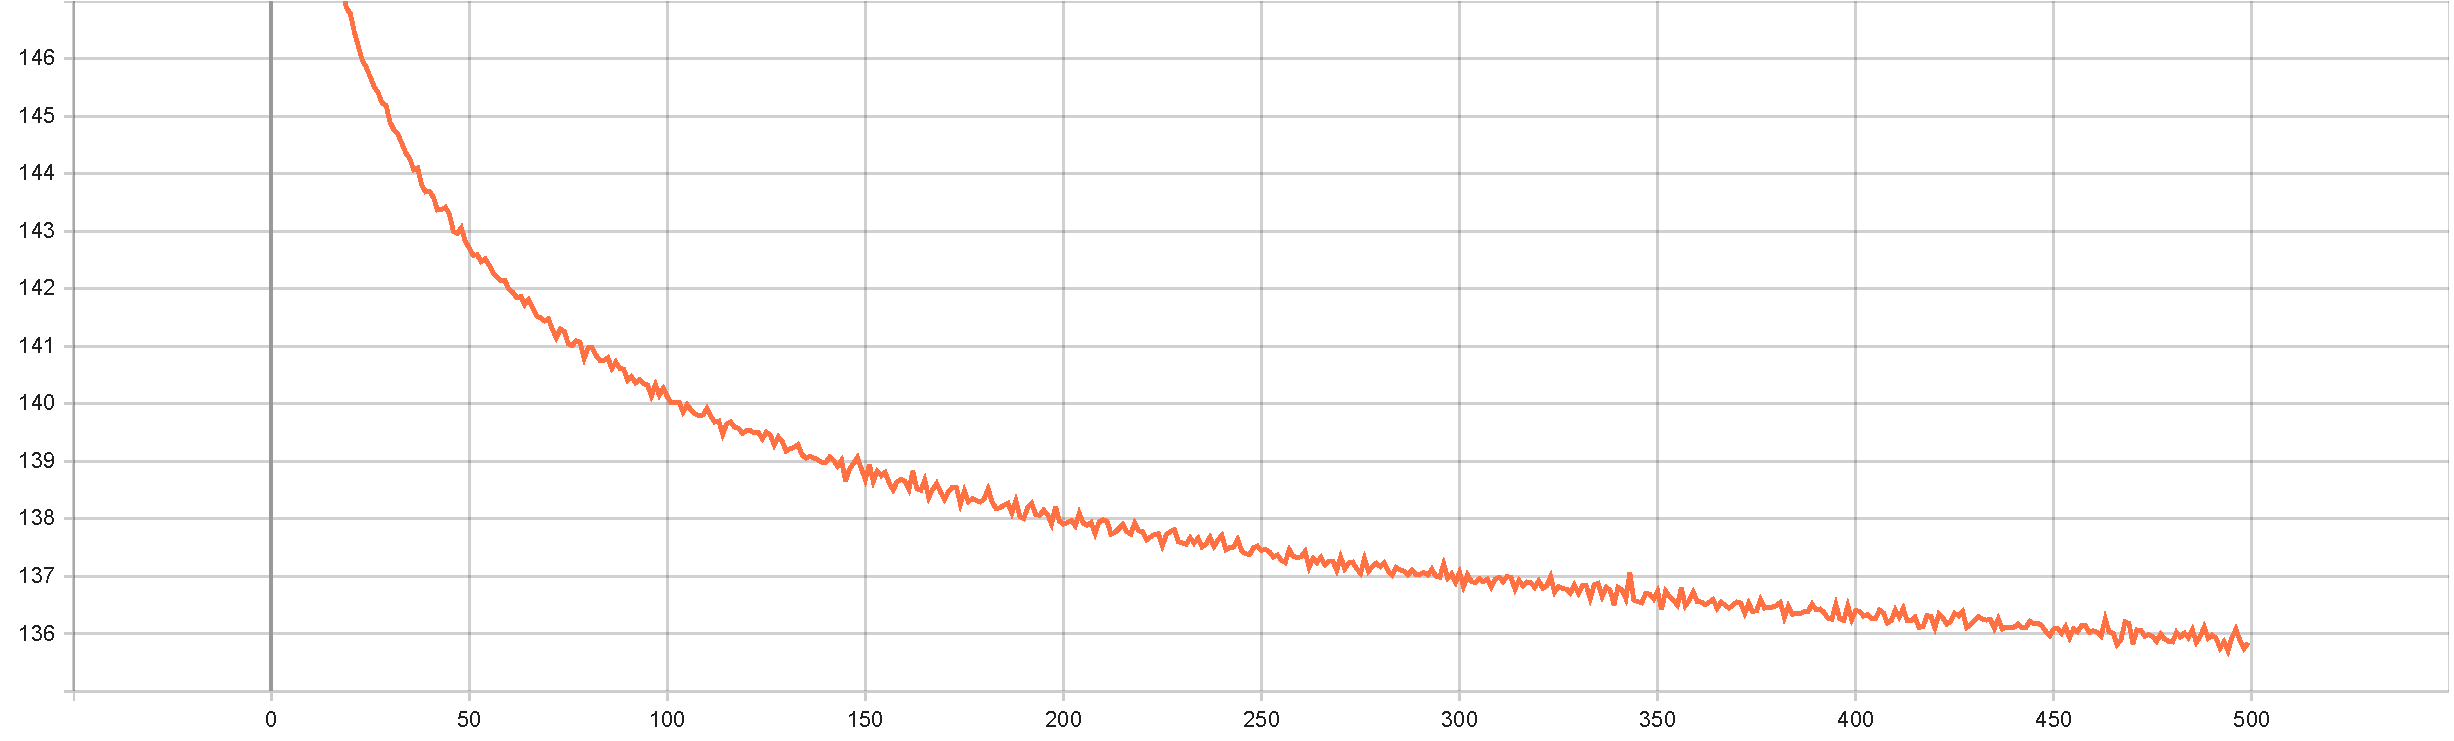
\includegraphics[width=0.97\textwidth]{figures/vae_model_total_loss_500_epochs.pdf}
    \caption{Ztrátová funkce po 500 epochách konverguje k hodnotě $\sim 135.8$. Osa x značí počet epoch. Osa y značí hodnotu ztrátové funkce.}
    \label{fig:vae_model_loss_function_converence}
\end{figure}

\begin{figure}[H]
    \centering
    \subfloat[\centering KL divergence po 500 epochách konverguje k hodnotě $\sim 3.8$.]{{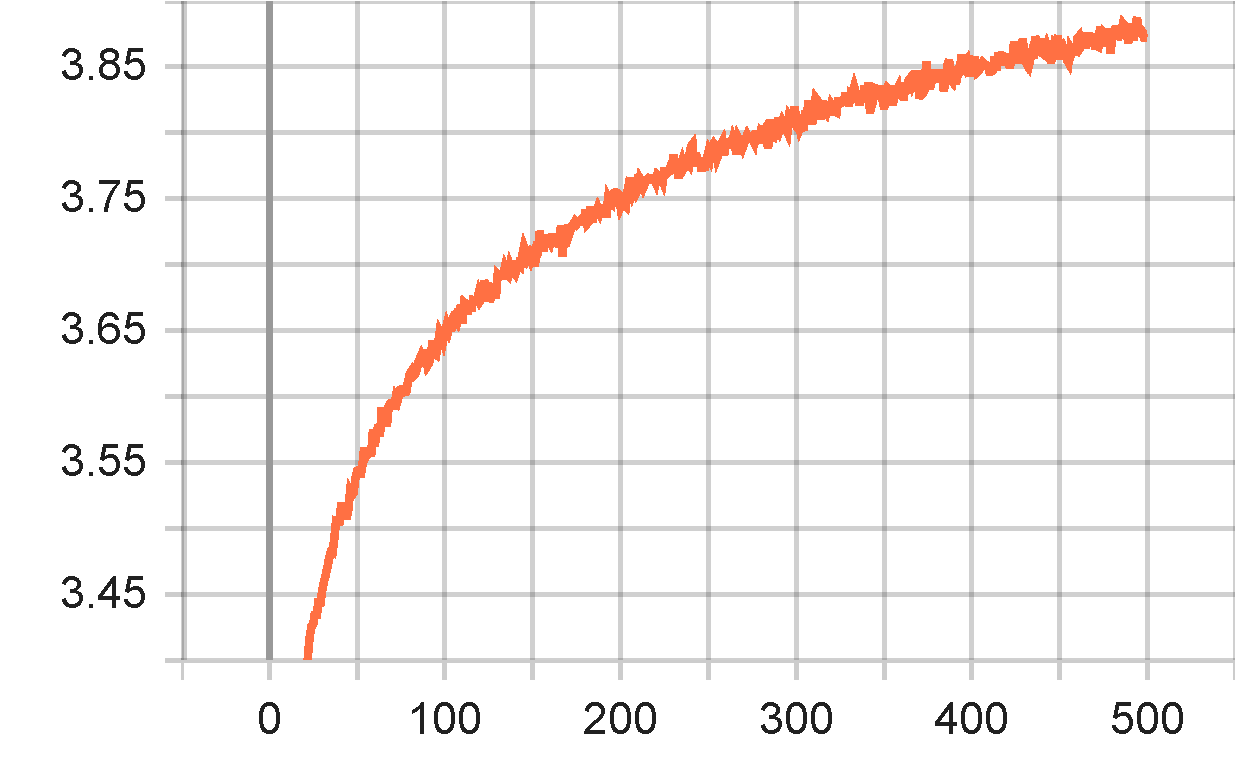
\includegraphics[width=0.45\textwidth]{figures/vae_model_kl_loss_500_epochs.pdf} }}
    \qquad
    \subfloat[\centering Chyba rekonstrukce po 500 epochách konverguje k hodnotě $\sim 132$.]{{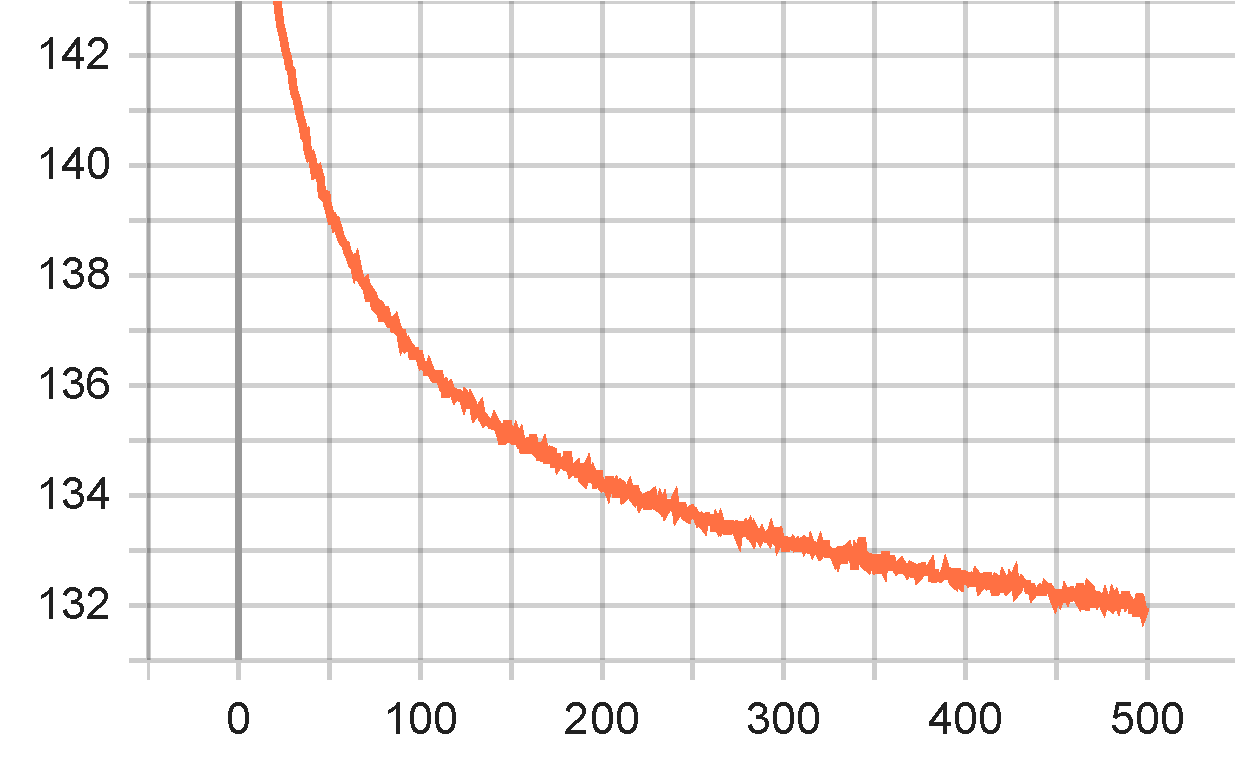
\includegraphics[width=0.45\textwidth]{figures/vae_model_reconstruction_loss_500_epochs.pdf} }}
    \caption{Hodnoty dílčích prvků ztrátové funkce modelu variačního autoenkodéru po 500 epochách. Osa x značí počet epoch. Osa y značí hodnotu dílčího prvku ztrátové funkce.}
    \label{fig:vae_model_loss_function_terms_converence}
\end{figure}

Celkový počet epoch byl stanoven základě doménové znalosti (tedy předem známý počet tříd, jejich sémantika a společné rysy) a postupného formování latentního prostoru, jak zachycuje \autoref{fig:forming_latent_space}.
Při vizualizaci latentního prostoru modelu, jehož trénovací fáze zahrnovala 500 epoch, lze pozorovat emergenci struktury jeho bodů, která \textbf{koresponduje se skutečným významem trénovacích dat} (číslice 0-9, 10 dostatečně izolovaných skupin).
Hodnota ztrátové funkce je při takovémto počtu epoch stabilizována a osciluje kolem celkové hodnoty $135.8$. Vývoj hodnot ztrátové funkce skrze různý počet epoch v trénovací fázi prezentuje \autoref{app:loss_function_development}.
V důsledku těchto jevů byla \textbf{trénovací fáze modelu ukončena} a uspokojivý \textbf{počet epoch trénovací fáze byl stanoven na 500}.

\subsection{Možné zlepšení trénovací strategie variačního autoenkodéru}
Variační autoenkodér při trénování balancuje dva prvky ztrátové funkce (viz \autoref{eq:vae_elbo}) – chybu rekonstrukce a KL divergenci.
Usměrnění těchto dvou prvku lze dosáhnout zahrnutím hyperparametru $\beta$ do trénovací fáze modelu. 
Tento hyperparametr má skalární hodnota a slouží k násobení KL divergence prvku ztrátové funkce, tedy přiděluje KL divergenci váhu \cite{Higgins2022}.

Je-li $\beta = 1$, pak variační autoenkodér optimalizuje efekt chyby rekonstrukce i KL divergence rovnocenně.   
Je-li $\beta < 1$, dává variační autoenkodér větší důraz na minimalizaci chyby rekonstrukce.
Je-li $\beta > 1$, dává variační autoenkodér naopak větší důraz na regularizační efekt KL divergence \cite{Higgins2022}.

V této ilustrační implementaci generativního modelu MNIST pro jednoduchost \textbf{hyperparametr $\beta$ nebyl součástí trénovacího procesu}.
Jeho začlenění by však dle \textcite{Higgins2022} vedlo k ještě lépe strukturovanému latentnímu prostoru naučeného modelu, než prezentuje \autoref{fig:forming_latent_space}.

U složitějších modelů variačního autoenkodéru nalézá uplatnění $\beta$ hyperparametru úspěch.
Výzkumníci \textcite{Sankarapandian2021} dokonce přichází se strategií postupného žíhání hodnoty $\beta$.
Začínají s hodnotou $\beta \ll 1$ a postupně ji zvyšují.
To v důsledku umožní modelu se v úvodní fázi trénování zaměřit na minimalizaci chyby rekonstrukce.
V pozdější fázi trénovacího procesu je naopak postupně upřednostňován regularizační efekt KL divergence, což ve finále vede k přesnějšímu zachycení struktury dat a zamezuje přeučení.

